% Protocol figure: Input -> Context Selector (ours, trained) -> Frozen LLM -> Review Findings.
% Layout after LLMLingua (Jiang et al., 2023, Fig. 1). Content is one real AACR-Bench PR,
% FreeCAD/FreeCAD#21257: diff lines, paths, counts and per-level input tokens are real values;
% the chosen level (L04) is illustrative, and the findings show the Codex /review JSON schema
% with placeholder values. Build: latexmk -pdf protocol.tex
\documentclass[tikz,border=4pt]{standalone}
\usepackage[T1]{fontenc}
\usepackage[default]{sourcesanspro}
\usepackage[scaled=0.86]{beramono}
\usepackage{amsmath,amssymb}
\usepackage{fontawesome5}
\usetikzlibrary{calc,arrows.meta,backgrounds,positioning}

% ---------------------------------------------------------------- palette
% Neutral warm greys for input and output, deep teal for our model, muted indigo for the
% frozen LLM, and one coral accent for the chosen context and its path.
\definecolor{ink}{HTML}{1F2328}   \definecolor{grey}{HTML}{6E6A65}  \definecolor{hair}{HTML}{DEDAD4}
\definecolor{inS}{HTML}{5C5751}   \definecolor{inF}{HTML}{FAF9F7}
\definecolor{ourS}{HTML}{2E7D78}  \definecolor{ourF}{HTML}{EDF6F5}  \definecolor{ourD}{HTML}{1F5E5A}
\definecolor{ourB}{HTML}{B5D8D4}
\definecolor{llmS}{HTML}{4F5D8C}  \definecolor{llmF}{HTML}{F1F2F8}
\definecolor{outS}{HTML}{5C5751}  \definecolor{outF}{HTML}{FAF9F7}
\definecolor{accC}{HTML}{E06A4E}
\definecolor{lblG}{HTML}{2E7D78}  \definecolor{lblR}{HTML}{B4473A}  \definecolor{lblB}{HTML}{4F5D8C}
\definecolor{addC}{HTML}{2F7D4F}  \definecolor{delC}{HTML}{C0392B}

\tikzset{
  >={Latex[length=2.6mm,width=2.1mm]},
  column/.style 2 args={draw=#1, fill=#2, line width=0.9pt, rounded corners=8pt},
  title/.style={font=\large\bfseries, anchor=north west, inner sep=0pt},
  sub/.style={font=\footnotesize, text=grey, anchor=north west, inner sep=0pt},
  card/.style={draw=hair, fill=white, line width=0.7pt, rounded corners=5pt},
  cardhead/.style={font=\small\bfseries, text=ink, anchor=north west, inner sep=0pt},
  main/.style={->, line width=1.5pt, draw=ink, rounded corners=4pt},
  inner/.style={->, line width=1.1pt, draw=ourD, rounded corners=3pt},
}
\newcommand{\dl}[1]{\textcolor{delC}{#1}}
\newcommand{\al}[1]{\textcolor{addC}{#1}}

\begin{document}
\begin{tikzpicture}
\def\top{0}\def\bot{-7.75}
\def\rowY{-4.205}   % y of the chosen level; the main output arrows run along it

% ======================================================================== 1  Input
\draw[column={inS}{inF}] (0,\top) rectangle (4.7,\bot);
\node[title, text=inS] at (0.3,-0.3) {Input};

\draw[card] (0.25,-0.95) rectangle (4.45,-4.75);
\node[cardhead] at (0.45,-1.12) {{\color{inS}\faFile*}\; Prompt};
\node[anchor=north west, text width=4.0cm, align=left, inner sep=0pt, font=\scriptsize, text=ink] at (0.45,-1.6) {%
  \textcolor{lblG}{\bfseries Instruction}\; Codex \texttt{/review} rubric + review request\\[3pt]
  \textcolor{lblR}{\bfseries PR}\; PartDesign: Fix hole centered on point edge case\\[3pt]
  \textcolor{lblB}{\bfseries Diff}\\[1pt]
  {\ttfamily\fontsize{5.0}{6.6}\selectfont
  \textcolor{grey}{ExportOCAF2.cpp @@ -381,7 +381,11 @@}\\
  \dl{- auto shape = Part::Feature::getTopoShape(}\\
  \dl{-~~~~parentObj, sub, false, nullptr, \&obj,}\\
  \al{+~~~~parentObj, sub, nullptr, \&obj,}\\
  \al{+~~~~Part::Feature::Transform * (!sub));}\\
  \textcolor{grey}{\ldots\ 25 files, 78 hunks}}};
\node[font=\scriptsize, text=grey, anchor=south east, inner sep=0pt] at (4.3,-4.6) {13,071 tokens};

\draw[card] (0.25,-5.0) rectangle (4.45,-7.5);
\node[cardhead] at (0.45,-5.17) {{\color{inS}\faFolderOpen}\; Project folder};
\node[anchor=north west, text width=3.85cm, align=left, inner sep=0pt, font=\ttfamily\fontsize{5.8}{7.6}\selectfont, text=ink] at (0.45,-5.65) {%
  FreeCAD/ \textcolor{grey}{\rmfamily\sffamily\scriptsize at the reviewed commit}\\
  \hspace*{2.2mm}\textcolor{grey}{\faFolder}~src/Mod/Part/App/\\
  \hspace*{4.4mm}\textcolor{grey}{\faFile[regular]}~PartFeature.cpp\\
  \hspace*{2.2mm}\textcolor{grey}{\faFolder}~src/Mod/PartDesign/App/\\
  \hspace*{4.4mm}\textcolor{grey}{\faFile[regular]}~FeatureHole.cpp\\
  \hspace*{2.2mm}\textcolor{grey}{\ldots}};
\node[font=\scriptsize, text=grey, anchor=south east, inner sep=0pt] at (4.3,-7.35) {135k symbols};

% ======================================================================== 2  Context selector (ours)
\draw[column={ourS}{ourF}] (5.4,\top) rectangle (12.0,\bot);
\node[title, text=ourD] at (5.7,-0.3) {Context Selector};
\node[sub, anchor=base west] at (8.95,-0.62) {(ours, trained)};

% I  trace
\draw[card, draw=ourB] (5.65,-0.95) rectangle (9.6,-2.5);
\node[cardhead] at (5.85,-1.12) {I\quad Code-graph trace};
\node[anchor=north west, inner sep=0pt, font=\scriptsize, text=grey, align=left, text width=2.3cm] at (5.85,-1.55)
  {45 changed symbols $\to$ callers, callees, tests, docs};
\coordinate (traceW) at (5.65,-1.65);
% mini code graph: the changed symbol (centre) and its neighbours in the code graph
\begin{scope}[shift={(9.0,-1.88)}, scale=0.55]
  \foreach \a in {0,60,...,300}{\coordinate (o\a) at (\a+30:0.8);}
  \foreach \a in {0,60,...,300}{\pgfmathtruncatemacro{\b}{mod(\a+60,360)}\draw[ourB, line width=0.8pt] (o\a) -- (o\b);}
  \foreach \a in {0,60,...,300}{\draw[ourS!70, line width=0.9pt] (0,0) -- (o\a);}
  \foreach \a in {0,120,240}{\fill[ourS] (o\a) circle (0.15);}
  \foreach \a in {60,180,300}{\fill[white] (o\a) circle (0.15); \draw[ourS, line width=0.9pt] (o\a) circle (0.15);}
  \fill[ourD] (0,0) circle (0.25);
\end{scope}


% selector
\node[circle, fill=ourD, text=white, minimum size=1.5cm, align=center, font=\small\bfseries] (sel) at (11.05,-1.72)
  {Selector\\[-3pt]$f_\theta$};
\draw[inner] (9.6,-1.72) -- (sel.west);

% II  ten nested levels with the PR's real input-token counts
\draw[card, draw=ourB] (5.65,-2.72) rectangle (11.75,-6.1);
\node[cardhead] at (5.85,-2.88) {II\quad Ten nested contexts \textmd{\color{grey}\footnotesize input tokens}};
\draw[inner] (7.2,-2.5) -- (7.2,-2.72);
\def\bx{7.55}
\foreach \i/\n/\t/\lab in {1/L01 diff/13.071/13k, 2/L02 + functions/40.921/41k, 3/L03 + files/64.103/64k,
                         4/L04 + callees/78.203/78k, 5/L05 + callers/86.864/87k, 6/L06 + tests/86.864/87k,
                         7/L07 + guides/91.080/91k, 8/L08 2 hops/118.289/118k, 9/L09 + docs/118.574/119k,
                         10/L10 all/256.337/256k}{
  \pgfmathsetmacro{\yy}{-3.35-0.285*(\i-1)}
  \pgfmathsetmacro{\ww}{3.15*\t/256.337}
  \ifnum\i=4
    \fill[accC, rounded corners=1.5pt] (\bx,\yy-0.1) rectangle ++(\ww,0.2);
    \node[font=\scriptsize\bfseries, text=accC, anchor=west, inner sep=2pt] at (\bx+\ww,\yy) {\lab};
    \node[font=\scriptsize\bfseries, text=accC, anchor=east, inner sep=0pt] at (\bx-0.1,\yy) {\n};
  \else
    \fill[ourB, rounded corners=1.5pt] (\bx,\yy-0.1) rectangle ++(\ww,0.2);
    \node[font=\scriptsize, text=grey, anchor=west, inner sep=2pt] at (\bx+\ww,\yy) {\lab};
    \node[font=\scriptsize, text=ink, anchor=east, inner sep=0pt] at (\bx-0.1,\yy) {\n};
  \fi
}
\draw[->, line width=1.1pt, draw=accC, dash pattern=on 4pt off 2.5pt, rounded corners=3pt]
  (sel.south) -- (sel.south |- 0,\rowY+0.0) -- (\bx+3.15*78.203/256.337+0.62,\rowY);
\node[font=\scriptsize\bfseries, text=accC, anchor=east] at (10.85,-3.4) {picks one};

% III  training
\draw[card, draw=ourB] (5.65,-6.3) rectangle (11.75,-7.5);
\node[cardhead] at (5.85,-6.47) {III\quad Trained offline};
\node[anchor=north west, inner sep=0pt, font=\scriptsize, text=grey, text width=5.7cm, align=left] at (5.85,-6.85)
  {on frozen-LLM reviews of every level, scored against human review comments};

% ======================================================================== 3  Frozen LLM
\draw[column={llmS}{llmF}] (13.75,\top) rectangle (16.85,\bot);
\node[title, text=llmS] at (14.05,-0.3) {Frozen LLM};
\node[card, draw=llmS!45, minimum width=2.45cm, minimum height=2.5cm, align=center, font=\footnotesize] (llm) at (15.3,\rowY)
  {{\fontsize{24}{26}\selectfont\color{llmS}\faSnowflake}\\[5pt]
   \textbf{\small Qwen3.8-27B}\\[1pt] {\color{grey}greedy, one call}\\ {\color{grey}weights not trained}};
\node[font=\scriptsize, text=grey, align=center] at (15.3,-6.9) {any LLM reviewer\\can be plugged in};

% ======================================================================== 4  Output
\draw[column={outS}{outF}] (17.55,\top) rectangle (22.35,\bot);
\node[title, text=outS] at (17.85,-0.3) {Review Findings};
\draw[card] (17.8,-2.3) rectangle (22.1,-6.1);
\node[anchor=north west, inner sep=0pt, align=left, font=\ttfamily\fontsize{5.6}{8.4}\selectfont, text=ink] at (18.0,-2.6) {%
  \{"findings": [\{\\
  \hspace*{2mm}"title": "\textless{}imperative, $\leq$80 chars\textgreater",\\
  \hspace*{2mm}"body": "why it is a problem \ldots",\\
  \hspace*{2mm}"priority": 1,\\
  \hspace*{2mm}"confidence\_score": 0.7,\\
  \hspace*{2mm}"code\_location": \{\\
  \hspace*{4mm}"absolute\_file\_path":\\
  \hspace*{6mm}"\ldots/Part/App/PartFeature.cpp",\\
  \hspace*{4mm}"line\_range": \{\ldots\}\}\},\\
  \hspace*{2mm}\ldots],\\
  \hspace*{0mm}"overall\_correctness": "\ldots"\}};
\node[font=\scriptsize, text=grey, align=left, anchor=north west, inner sep=0pt] at (17.85,-6.3)
  {Codex \texttt{/review} JSON schema;\\values are placeholders};

% ======================================================================== main arrows
\draw[main] (4.45,-1.65) -- (traceW);
\draw[main] (4.45,-6.15) -- (5.0,-6.15) -- (5.0,-1.95) -- (5.65,-1.95);
\draw[main, draw=accC] (11.75,\rowY) -- node[font=\scriptsize\bfseries, text=accC, above=2pt, align=center, pos=0.45]{prompt + $C_4$\\{\mdseries 78k tokens}} (llm.west);
\draw[main] (llm.east) -- (17.8,\rowY);

\end{tikzpicture}
\end{document}
